\RequirePackage{nag}
\documentclass[12pt,letterpaper]{article}
\usepackage{atbegshi}
\usepackage{lipsum}

% \usepackage{fixltx2e}
% \usepackage{classicthesis}
\usepackage{polyglossia}
\usepackage[natbib=true, 
			style=numeric, %authoryear or numeric; comp == compact
			bibstyle=nature, 
			backend=biber,
			uniquelist=false, 
			sorting=none,
			uniquename=false]{biblatex}
\usepackage{booktabs}
\usepackage{relsize}
\usepackage{setspace}
\usepackage{lineno}
\usepackage{wrapfig}
\usepackage{sidecap}

\setdefaultlanguage{english}
\setmainfont[Mapping=tex-text, 
			 Numbers=OldStyle, 
			 % SizeFeatures={{Size=12}}
			 ]{Times}
\setsansfont[Mapping=tex-text, 
			 Numbers=OldStyle, 
			 % SizeFeatures={{Size=12}}
			 ]{Helvetica}
\setmonofont[Scale=0.8]{Monaco}
\setcounter{secnumdepth}{0}

\addbibresource{ELI.bib}

% Set the line spread (height). Be careful here, use too small rather than too
% large value. Also: double-spaced lines correspond to a value of ~1.3,
% depending on the font, NOT to 2.0
\setstretch{1.1} % 1.1 normally

\graphicspath{{figs/}}

%% Custom macros

\newcommand*\captitle[1]{\textbf{#1}}
\newcommand*\todo[1]{%
    \graffito{\textcolor{red}{TO\ DO: #1}}}

\newcommand*\gene[1]{\textit{#1}}
\newcommand*\ko[1]{\textit{#1\textsuperscript{\(-/-\)}}}
\newcommand*\protein[1]{#1}
\newcommand*\species[1]{\textit{#1}}


\title{\ruleline{Project Narrative}}
\lhead{Zhian N. Kamvar, Ph. D.}
\rhead{Project Narrative}

\begin{document}
\maketitle
% \linenumbers

\section{Training/Career Development Plan}

% The Training/Career Development Plan is a description of all activities that
% the applicant plans to perform and participate to enhance the pre- or
% postdoctoral training during the fellowship award period.

% For Postdoctoral Fellowship applicants, a Training/Career Development Plan
% includes plans for transition to career independence by development of
% professional skills. These professional skills include teaching competencies;
% what those career and training goals are; and results of the postdoctoral
% fellow's previous and current research and scholarships that include
% publications, presentations, etc.
\subsection{Personal Statement}

\begin{wrapfigure}[]{R}[]{0pt}
  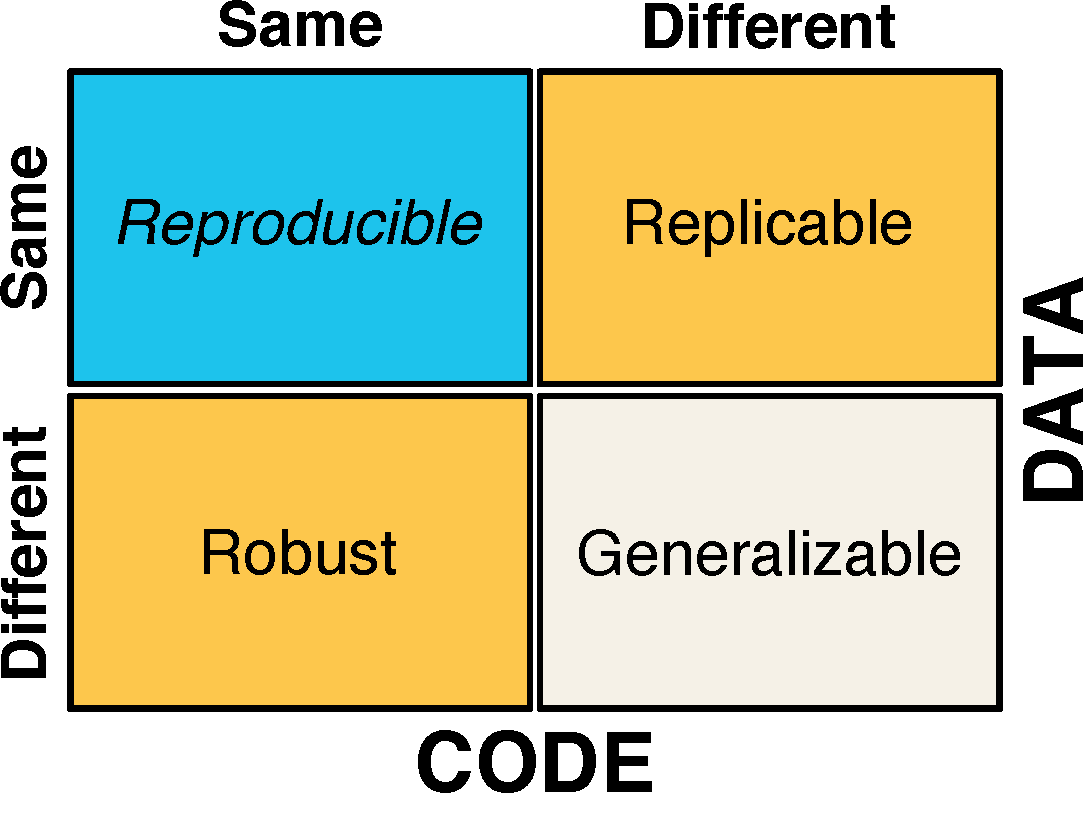
\includegraphics[width=0.35\textwidth]{figure/whitaker2017publishing.pdf}
  \caption{Conceptual definition of computational reproducible research (top left) adapted from \citet{whitaker2017publishing}. If the code and data are the same, they should produce the same results \citep{patil2016statistical}.}
  \label{fig:rr-def}
\end{wrapfigure}

My ultimate goal is to improve the field of agricultural research by demonstrating the value of open and reproducible research (Fig. \ref{fig:rr-def}) in the form of workshops and course curriculum. 
There are numerous, well documented benefits to open and reproducible research \citep{mckiernan2016open}, and, in recent years, a lack of reproducibility in psychological and biomedical studies have been labeled a ``reproducibility crisis'' in the popular press \citep{baker2016scientists,patil2016statistical}. 

The proposed research aims to understand local adaptation of the plant pathogenic fungus \textit{Sclerotinia sclerotiorum} across thermal regions. 
By conducting this research openly, I can use the data and analyses as source materials to create educational activities. 
These will be focused on the topic of reproducible and open research in genomic data analysis, which will be taught as a special topics course in the Department of Plant Pathology at the University of Nebraska-Lincoln. 
A summary of the course will additionally be published in the journal \textit{Plant Health Instructor}. 
\textbf{My overall goals for this fellowship are to develop my skills in education and genomic-scale research.} 

\subsection{Research Training}

Broadly, my current research focuses on understanding the population dynamics and evolutionary processes governing the clonally-reproducing fungal pathogen \textit{S. scleroitoriorum}.
I use reproducible research practices for data analysis. 
My research has largely been focused on microsatellite data, and I have experience with genome assembly (i.e. by creating a make-based genome assembly pipeline: \url{https://github.com/zkamvar/read-processing}).
I do not have substantial experience asking evolutionary questions of large-scale genomic data. 
\textbf{The goal of research training} is to compliment my skills as a data scientist with the tools and techniques necessary for evolutionary genomic data analysis. 

\begin{itemize}
  \item \textbf{Background Training In: } population genetics, evolution, molecular techniques, microbiological techniques, and R programming
  \item \textbf{Experienced In: } reproducible research techniques, methods development, cluster computing, population genetic analysis, software development, multivariate analysis, sequence alignment
  \item \textbf{Inexperienced In: } coalescent analysis, Bayesian statistics, phylogeographic analysis
\end{itemize}

\subsubsection{Research Training Plan}

\begin{enumerate}
  \item \textbf{Workshop on Molecular Evolution at Woods Hole, MA:} this workshop consists of lectures, discussions, and bioinformatic exercises that span contemporary topics in molecular evolution. Training topics specific to my deficiencies include, but are not limited to: phylogenetic analysis (maximum likelihood theory and practice, Bayesian analysis; hypothesis testing), population genetics analysis (coalescence theory, maximum likelihood and Bayesian estimation of population genetic parameters), molecular evolution (gene duplication and divergence, gene family organization), and comparative genomics (genome content, structure, and evolution).
  \item \textbf{Preregistration:} A description of all data, analyses, and expectations will be described in a public preregistration submission to the Open Science Framework.
  \item \textbf{Collection of 96 \textit{S. sclerotiorum} isolates from China and US:} Isolates from four regions in China will be provided by Dr. Weidong Chen; those from four regions in the US will be provided by Dr. James Steadman. 
  \item \textbf{DNA Extraction and Illumina Sequencing:} Genomic DNA will be extracted under the supervision of Dr. Sydney E. Everhart and sent for library preparation and sequencing at the Beijing Genome Institute (BGI). 
  \item \textbf{Data Validation and Analysis:} Genome assembly, data validation,
  and analysis will be done on the Holland Computing Center (HCC) Clusters at University of Nebraska-Lincoln. Genome sequences will be deposited in GenBank and all metadata and analysis scripts will be stored at the Open Science Framework and given a unique Digital Object Identifier.
\end{enumerate}


\subsection{Pedagogical Training}

I have experience teaching short, 3 hour workshops, but don't have formal training in pedagogical methods beyond my training as a Teaching Assistant for a 200 level introductory biology course. 

\begin{itemize}
  \item \textbf{Background Training In: } Assignment evaluation, laboratory section management
  \item \textbf{Experienced In: } Interactive laboratory instruction, K-12 English as a Foreign Language instruction, Short-form workshop development and
  instruction
  \item \textbf{Inexperienced In: } Active learning techniques, course creation and evaluation, developing goals for specific learning outcomes, course portfolio development
\end{itemize}

\subsubsection{Pedagogical Training Plan}

\begin{enumerate}
  \item \textbf{Workshop training} will be provided by Data Carpentry. In my first year, I aim to complete instructor training and certification.
  \item \textbf{Northstar Summer Institute for Scientific Teaching:} This workshop in Twin Cities, MN will cover tools and techniques for scientific teaching. These include modes of assessment, backward design, creating and sustaining inclusive environments, the use of current education literature for course improvement.
  \item \textbf{Course Development:} Development of the reproducible research course will begin immediately by defining public data sets to use as examples and developing basic materials for reproducible research.
  \item \textbf{Special Topics Course in Plant Pathology at UNL:} I will create a three credit-hour special topics course about reproducible research. This will be held in the department of Plant Pathology and offered to anyone in the agricultural sciences. 
\end{enumerate}


\subsection{Career Development}

\begin{itemize}
  \item \textbf{Background Training In: } manuscript preparation, peer-review process, research ethics, outreach methods
  \item \textbf{Experienced In: } professional writing (CV, r\'esum\'e, cover letters), written and oral communication of scientific research to professional and lay audiences, leadership
  \item \textbf{Inexperienced In: } research grant writing, course development, grant budget management, inter-organizational leadership
\end{itemize}

\subsection{Career Development Plan}

\begin{enumerate}
  \item \textbf{Professional Development} in writing grant proposals, and grant-budget management will be provided under the guidance of Dr. Sydney E. Everhart.
  \item \textbf{Develop five-year plan} for future projects, funding sources, and jobs including applications to tenure-track faculty positions.  
\end{enumerate}

% ------------------------------------------------------------------------------


\section{Mentoring Plan}

The applicants are expected to engage their mentors and/or advisors in the
development of their application. Thus, prior to submission of the
application, prospective fellows should already identify a Primary mentor who
will be willing to help them in their projects as well as professional
development (note: more than one Primary Mentor is acceptable for Integrated
Projects Only). If there are other collaborating mentors, their role and
responsibilities to the project and development of the applicant's skills
should be clearly described. For predoctoral applications, if the primary
mentor is not the student's graduate advisor or laboratory sponsor, the
relationship between advisor's work and the primary mentor's research should
be clearly defined, and the contribution of each individual in the student's
project as well as degree completion should be included. Because this is a
very important component of the project, the commitment of the mentor(s) is
included in the evaluation criteria as it pertains to project personnel. In
describing the role of the mentor, the applicant should:

\begin{enumerate}

  \item Briefly indicate how the mentoring and educational training will add to the
   skill sets of the National Institute of Food and Agriculture (NIFA) Fellow.

  \item Briefly explain the commitment of the primary mentor.

  \item Briefly describe the role of collaborating mentors (if applicable).

  \item With respect to the Primary Mentor, provide a list of former mentees and
   their current positions. 
   \begin{quote}
   NOTE: The Primary Mentor shall submit a Letter of Commitment (as an
   attachment to Field 12, Other Attachments, of the Other Project
   Information form-see section g. in the AFRI ELI RFA) explicitly
   indicating their respective responsibilities throughout the proposed
   project in relation to the Project Director.
   \end{quote}

  \item Briefly list and explain the role of other non-primary mentors.

\end{enumerate}


\section{Project Plan}

% The research should be totally independent of the mentor's. Proven techniques
% and technologies as part of the experimental approach, especially if these are
% routinely employed, don't have to be provided in detail. Experimental
% approaches or strategies including possible pitfalls and alternatives must be
% provided in order to assess the overall feasibility of the Updated March 10,
% 2017 proposed study. Avoid open-ended screens or undefined outcomes. The scope
% of the project should be within the 2-year timeframe.

\subsection{Introduction}

% \begin{figure}[htbp]
%   \centering
%   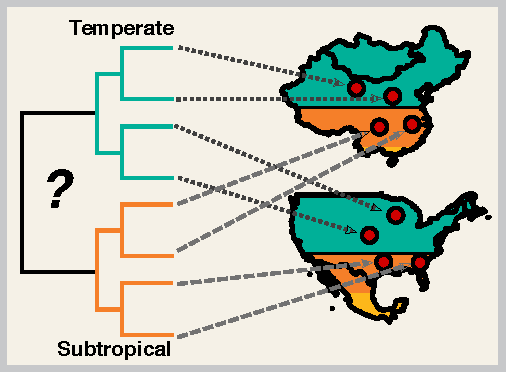
\includegraphics[width=0.35\textwidth]{figure/us-china.pdf}
%   \caption{A hypothesis of the evolutionary history of \textit{S. slcerotiorum} in temparate and subtropical regions between North America and East Asia}
%   \label{fig:us-china}
% \end{figure}

% \begin{SCfigure}[][htbp]
%   \centering
%   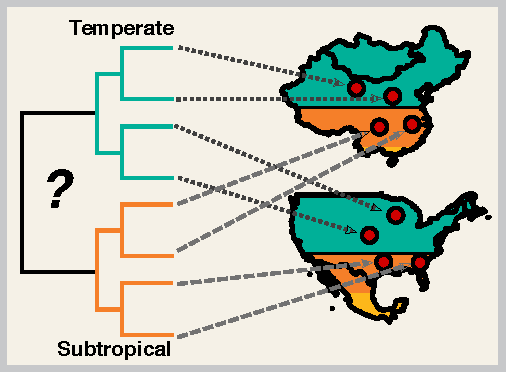
\includegraphics[width=0.35\textwidth]{figure/us-china.pdf}
%   \caption{A hypothesis of the evolutionary history of \textit{S. slcerotiorum} in temparate and subtropical regions between North America and East Asia}
%   \label{fig:us-china}
% \end{SCfigure}






% The introduction should include a well-defined problem, a clear statement of
% the long-term goal(s), and supporting objectives of the proposed project.
% Summarize the body of knowledge or other past activities that substantiate the
% need for the proposed project. Describe ongoing or recently completed
% activities related to the proposed project including the work of key project
% personnel. Include preliminary data/information pertinent to the proposed
% work. All works cited should be referenced (see Bibliography \& References
% Cited, see section d. in the AFRI ELI RFA).\\
% \rule{\textwidth}{0.5pt}

\textit{Sclerotinia sclerotiorum} is a cosmopolitan, haploid, plant pathogenic soil fungus with over 400 hosts worldwide \citep{bolton2006sclerotinia} and causes up to \$252M in losses per year on sunflower, soybeans, dry edible beans, canola, and pulse crops \citep{uscanola}. 
Significant levels of differentiation have been found between populations on canola in the United States (US) and China \citep{attanayake2013sclerotinia}, but these arise from different climate regions. 
Effective management strategies depend on the knowledge of genetic diversity and sexual reproduction \citep{grunwald2016population}.

Numerous studies over the last 30 years around the world show increased diversity in subtropical regions, but \citet{lehner2017sclerotinia} show that this may be an artifact of low resolution genetic markers.
Several studies have been conducted either across continental or climate regions, but no studies have addressed if the differences observed between \textit{S. sclerotiorum} populations is due to climate or region. 
\textbf{The two-pronged goal} of the proposed research is to \textbf{a)} determine if there is any potential for local adaptation to climate and \textbf{b)} develop a course on reproducible methods for genomic data analysis, using the research products as real world examples. 


\begin{wrapfigure}[]{R}[]{0pt} % [lineheight]{position}[overhang]{width}
  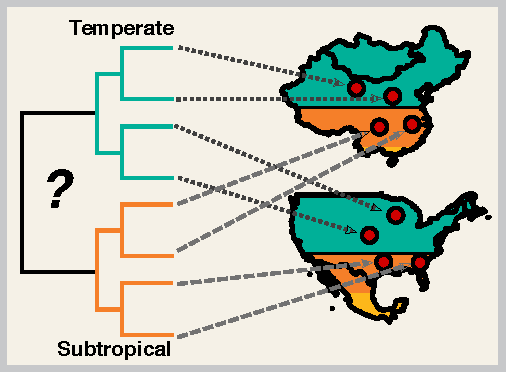
\includegraphics[width=0.35\textwidth]{figure/us-china.pdf}
  \caption{A hypothesis of the evolutionary history of \textit{S. slcerotiorum} in temparate and subtropical regions between North America and East Asia}
  \label{fig:us-china}
\end{wrapfigure}


\begin{wrapfigure}[]{l}[]{0pt}  % 8 if hanging on new page
  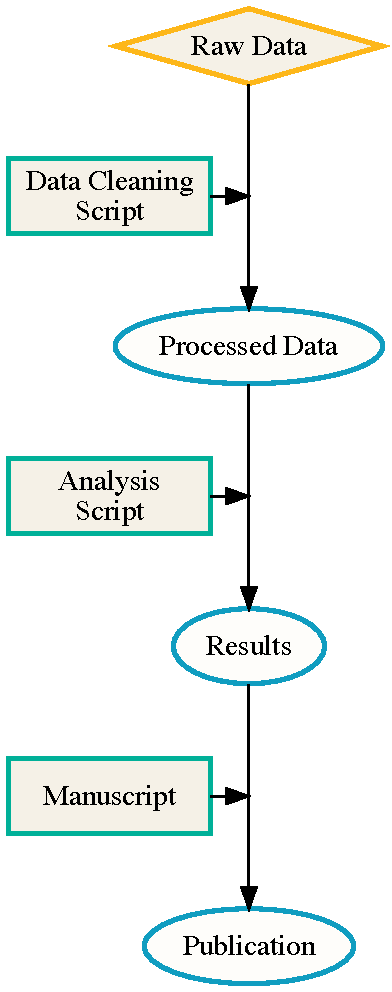
\includegraphics[width=0.35\textwidth]{figure/rr.pdf}
  \caption{An automated reproducible research workflow}
  \label{fig:rr}
\end{wrapfigure}

As genomic and microbiome data becomes more readily available, scientists with very little background in bioinformatics are conducting studies with no knowledge of how to process their data, which could lead to error-prone ad-hoc methods of data processing \citep{stewart-lowndes2017path, barone2017unmet}. 
There are many well-documented benefits to reproducible research including increased citation counts, funding opportunities, collaborations, etc. \citep{mckiernan2016open,stewart-lowndes2017path}.\\
\textbf{Objective \#1:} Perform whole genome sequencing on 96 isolates collected hierarchically over 8 subpopulations in North America and East Asia, respectively (Fig. \ref{fig:us-china}).\\
% \textbf{Objective \#2:} Perform reciprocal common garden laboratory experiments to evaluate fitness in different thermal environments.\\
\textbf{Objective \#2:} Perform phylogeographic and coalescent analyses to determine if divergence is due to climate or geography.\\
\textbf{Objective \#3:} Use the research products of objectives 1 \& 2 to create educational materials for graduate students that covers topics from
data validation and curation, method choice, version control, and open data science practices (Fig. \ref{fig:rr-def}, \ref{fig:rr}).

We plan to infer genetic diversity, migration patterns, and outcrossing with modern, reproducible population genetic and phylogeographic approaches on whole genome sequence data. 

The long-term goals of the research are to \textbf{a)} provide fine-scale knowledge of diversity within \textit{S. sclerotiorum} across climate regions within continents and \textbf{b)} to create educational materials for the training of graduate students in reproducible research. 




\subsection{Rationale and Significance}


% \begin{itemize}
%   \item Concisely present the rationale behind the proposed project and how it will
%   advance the current knowledge in the field;

%   \item Clearly describe the specific relationship of the project's objectives to
%   one of the Program Area Priorities. The Program Area Priority(ies) must be
%   specifically identified
% \end{itemize}

% connects proposal to purpose of grant program
% relates proposal to purpose of UNL
% states need in terms of end users. 

%  AFRI Foundational Priority for....
    % - Plant health and production and plant products;
    % - Animal health and production and animal products;
    % - Food safety, nutrition, and health;
    % - Bioenergy, natural resources, and environment;
    % - Agriculture systems and technology;
    % - Agriculture economics and rural communities
\noindent
\textbf{AFRI Foundational Priority for Plant Health and Production and Plant Products}

The rationale of the proposed work is that 1) the identification of patterns for adaptation in \textit{S. sclerotiorum} will reduce inputs by influencing management decisions regarding movement of inoculum, 2) genomic data and analyses from 96 isolates of \textit{S. sclerotiorum} will help drive novel research on this cosmopolitan pathogen, and 3) producing educational materials on open and reproducible research will have long-term benefits for agricultural research by increasing access to eduction and emphasizing practices that will positively influence stakeholder confidence and provide a wealth of knowledge from open future data and materials. 

The practice of open and reproducible research has been shown to increase the speed and accuracy of which scientific research is conducted \citep{stewart-lowndes2017path, wilson2016good}.
Surveys conducted in 2016 showed that 90\% of researchers acknowledge a reproducibility crisis in science \citep{baker2016scientists} and that the most pressing need is for training on data management and integration \citep{barone2017unmet}. 
Calls for conscious efforts to increase reproducibility have been around for many years \citep{buckheit1995wavelab, peng2011reproducible}, but only recently has training been emphasized \citep{schmidt2016stepping, stewart-lowndes2017path, wilson2016good}. 
By training graduate students seeking masters or doctoral degrees on how to perform open and reproducible research, future agricultural science will be cost effective, innovative, and engaging. 
This is in line with the teaching mission of the University of Nebraska, where multidisciplinary graduate education is explicitly mentioned as a focal point.

Canola production is a growing industry in the United States, producing 3 billion pounds of seed grossing at \$500 million in 2016 \citep{usda2017production, usda2017values}. Losses due to Sclerotinia Stem Rot are estimated to be 1\% yield for every 2\% disease incidence \citep{delrio2007impact}, and the midwest has seen an average incidence rate of 13\% \citep{markell2009sclerotinia}, which would mean an annual loss of \$30 million. 
It is known that local climate can exacerbate the spread of inoculum and thus, understanding the evolutionary potential for \textit{S. sclerotiorum} to adapt to a warming climate is essential for targeting future management decisions \citep{attanayake2014inferring,shea2000integrated,billiard2012sex}.

For over 15 years, population genetic analysis on \textit{S. sclerotiorum} has been performed using the same set of simple sequence repeat (SSR) markers \citep{sirjusingh2001characterization}. 
These markers, however, have been unable to accurately determine the number of unique genotypes in a sample \citep{lehner2017independently, lehner2017sclerotinia,arnaud2007standardizing}.
Moreover, these markers may suffer from confirmation bias, only able to describe the diversity of \textit{S. sclerotiorum} in the Midwestern United States \citep{attanayake2013sclerotinia}. 
Using whole genome sequences of representative isolates across continents allows us to capture a breadth of diversity, giving us a clear picture of the adaptive potential in \textit{S. sclerotiorum} \citep{grunwald2016population}.
By understanding the potential for thermal adaptation in \textit{S. sclerotiorum}, we can better predict how it will respond to changes in climate \citep{croll2016genetic}.


% Educational components must address one or two of the following key
% strategic actions:
% - Train students for Associate, Baccalaureate, Master's or Doctoral
% degrees; and/or
% - Prepare K-12 teachers and higher education faculty to understand and
% present food and agricultural scienc


\subsection{Approach}


% Provide a concise description of the proposed project and the problem(s) to be
% addressed. Clearly describe the approaches to be used. Specifically, this
% section must include:

% \begin{itemize}
%   \item A description of the project details proposed and the sequence in which the
%    activities are to be performed;
 
%   \item Methods to be used in carrying out the proposed project and feasibility of
%    the methods (detail only if a new and unproven method is to be used; if
%    employing commonly used methods provide information on the expertise
%    available);
 
%   \item Expected outcomes and outcome measures;
%   \item Means by which results will be analyzed, assessed, or interpreted;
%   \item How results or products will be used;
%   \item Pitfalls that may be encountered, and possible alternatives;
%   \item Limitations to proposed procedures;
 
%   \item A full explanation of any materials, procedures, situations, or activities
%    related to the project that may be hazardous to personnel, along with an
%    outline or precautions to be exercised to avoid or mitigate the effects of
%    such hazards;
 
%   \item A timeline for attainment of objectives and for production of deliverables
%    that includes annual milestones with specific, measurable outcomes; and
 
%   \item Establishment of a profile on an established professional social networking
%    site to document career progress during and beyond the duration of the
%    Fellowship.

% \end{itemize}


\subsubsection{Objective \#1: Whole Genome Sequencing of 96 \textit{Sclerotinia sclerotiorum} isolates}

\noindent \textbf{Methods for sampling -}
A total of 96 isolates split evenly across eight subpopulations of \textit{S. sclerotiorum} will be gathered from canola fields in China and the USA representing temperate regions temperate regions (between $40^{\circ}N$ and $66^{\circ}N$) and subtropical regions (between $23.5^{\circ}N$ and $40^{\circ}N$).
Isolates from China will be random samples from Gansu, Qinghai, Anhui, and Hunan provinces \citep{zhou2014dimethachlon, attanayake2013sclerotinia}.
Isolates from USA will be from canola fields in North Dakota, Colorado, Georgia, and South Carolina \citep{aldrich-wolfe2015genetic,phillips2002phylogeography}.\\
\noindent \textbf{Methods for sequencing -} 
Whole genomic DNA will be sequenced to >15X depth on a single lane of Illumina HiSeq 4000 sequencer and deposited in the UNL Attic data storage system. 
All isolates will be mapped to the \textit{S. sclerotiorum} reference genome using a workflow modified from \url{https://github.com/zkamvar/read-processing}, which uses \textsc{Bowtie2} and \textsc{Samtools} to map reads and \textsc{GATK} for variant discovery \citep{langmead2012fast, li2009sequence, mckenna2010genome, derbyshire2017complete}.\\ 
\noindent \textbf{Expectations -}
Based on preliminary results from sequencing clonal strains of \textit{S. sclerotiorum} after fungicide exposure we expect to see, on average, $\geq98.5\%$ coverage with $\geq8\times$ depth for all isolates. Because the reference genome of \textit{S. sclerotiorum} is from the US, we additionally expect a greater number of variants in the isolates from China.\\
\noindent \textbf{Pitfalls and Limitations -}
If the differentiation due to continent is sufficiently large, our alignments of the isolates from China may not efficiently align to the reference genome. 
We can monitor this by assessing mapping quality for all alignments and performing de-novo assembly on the isolates.

\subsubsection{Objective \#2: Assessment of Local Adaptation to Climate}

\noindent \textbf{Methods -} We will use phylogenetic data from each gene independently to assess the evolutionary history of these populations using \textit{Botrytis cinerea} as an outgroup \citep{staats2012genome}. 
To address phylogenetic incongruence, we will use a newly developed multivariate methods for exploring the space of phylogenetic trees across the genome \citep{kendall2016mapping, jombart2017treespace}. 
Adaptive potential will be assessed using ratios of synonymous and non-synonymous mutation rates, classifying them into positive, neutral, or negative selection, and comparing them to classes of tree topologies (geo-centric, climate-centric, or random) via $\Chi^2$ test.
Migration rates between populations will be assess using
Approximate Bayesian Computation with coalescent approaches. We will use \textsc{ABCtoolbox} to assess migration among climate and geographic regions \citep{wegmann2010abctoolbox}. 
Simulations will be carried out on each gene independently using the \texttt{msprime} simulator \citep{kelleher2016efficient}. 
Mean nucleotide diversity ($\pi$) and mean number of alleles will be used as summary statistics for evaluating simulations. 
Partial least squares regression and Euclidean distance to observed data will be utilized as the rejection method.\\
\noindent \textbf{Expectations -}
Based on initial data from \citet{attanayake2013sclerotinia}, I expect a majority of genes will segregate for geographic differentiation, but I predict that the majority of the positive selection will be found in the climate-centric genes, whereas the others will be majority neutral.\\
\noindent \textbf{Pitfalls and Limitations -}
If the samples are not true representatives of their populations, there exists a possibility for false positives for a signature of adaptation to climate.\\

\subsubsection{Objective \#3: Development of Education Modules on Open and Reproducible Research}

\noindent \textbf{Methods -} A course will be developed under the supervision of the Peer Review for Teaching Project at UNL (\url{http://peerreview.unl.edu/}). 
The course philosophy is that the student should not necessarily learn to use specific programs or languages, but to develop thought processes that allow them to adapt to new tools and workflows.
This course will be split up into four distinct sections, Philosophy of Open Science, Data Management, Best Practices in Reproducible Research, and Research Dissemination. 
Each of these three sections will draw from the data, analysis, and lessons learned in objectives 1 and 2.\\
\noindent \textbf{Expectations -}
I expect for the students to have a grasp of the overall philosophy and benefits of open and reproducible research.\\
\noindent \textbf{Pitfalls and Limitations -}
These students will likely be a self-selected group of students who are already interested in reproducible research, which would not necessarily beget any change in the field. To correct for this, I will design advertisements targeted at students from both applied and basic scientific research.\\

\noindent \textbf{Hazards -} No known hazards are associated with this project.

\noindent \textbf{Timeline - }

\section{Evaluation Plan}

A plan for evaluating progress towards objectives related to the
training/career development plan, mentoring plan, and project plan. The plan
must include milestones, which signify the completion of a major deliverable,
events, or accomplishment and serve to verify that the project is on schedule
and on track for successful conclusion. The plan should also include
descriptions of indicators that will be measured to evaluate whether the
education activities are successful in achieving project goals and contribute
to the achievement of the stated program goals and outcomes; and a
dissemination plan describing the methods that will be used to communicate
findings and project accomplishments.

In addition to the Project Narrative requirements above, the proposed
Integrated Project should clearly articulate:

\begin{itemize}

  \item Stakeholder involvement in project development, implementation, and
   evaluation, where appropriate;

  \item Objectives for each function included in the project (note that extension
   and education activities are expected to differ and to be described as
   separate project objectives; see enumerated descriptions in Part II, C
   (page 7 in the AFRI ELI RFA); and Updated March 10, 2017

  \item A dissemination plan describing the methods that will be used to
   communicate findings and project accomplishments.

  \item A plan for evaluating progress toward achieving project objectives must be
   included. The plan must include milestones, which signify the completion of
   a major deliverable, event, or accomplishment and serve to verify that the
   project is on schedule and on track for successful conclusion. The plan
   should also include descriptions of indicators that you will measure to
   evaluate whether the research, education, and/or extension activities are
   successful in achieving project goals and in contributing to achievement of
   the stated program goals and outcomes.

\end{itemize}


% https://tex.stackexchange.com/a/224803/77699
\newpage
\AtBeginShipout{%
\AtBeginShipoutDiscard
}

\printbibliography

\end{document}
